\chapter{Resultados e Discussões}

A Fig. \ref{clusterT1} apresenta à variação das propriedades físicas analisadas por agrupamento de classes de rochas para o poço T$1$. Em destaque, de vermelho, o litotipo diabásio. 

\begin{figure}[H]
	\centering
	\setlength{\fboxsep}{8pt}
	\setlength{\fboxrule}{0.1pt}
	\fbox{
		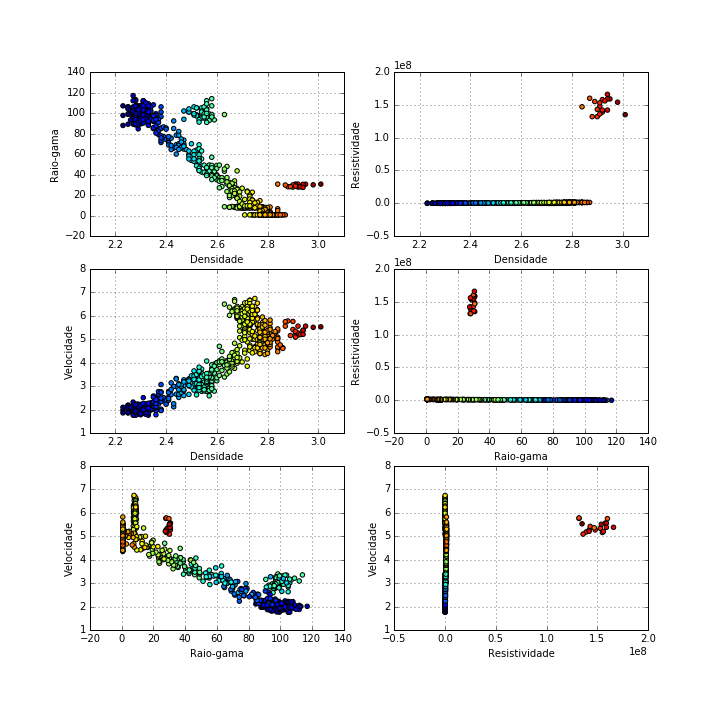
\includegraphics[scale=0.5]{Imagens/cluterpocoT1.png}
	}
	\caption{Agrupamento de dados do poço T1.}
	\label{clusterT1}
\end{figure} 

É perceptível o notável contraste de variação das propriedades físicas entre a rocha de origem ígnea, em contraste com as propriedades físicas das demais rochas de origem sedimentar e metamórfica. 

A Fig. \ref{clusterC1} apresenta à variação das propriedades físicas analisadas por agrupamento de classes de rochas para o poço C$1$. Em destaque, de vermelho, o litotipo diabásio. 

\begin{figure}[H]
	\centering
	\setlength{\fboxsep}{8pt}
	\setlength{\fboxrule}{0.1pt}
	\fbox{
		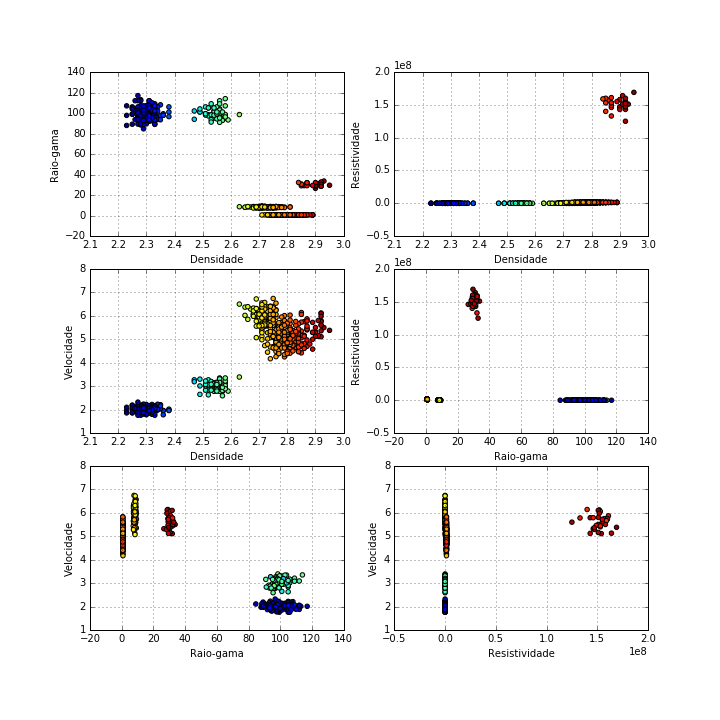
\includegraphics[scale=0.5]{Imagens/cluterpocoC1.png}
	}
	\caption{Agrupamento de dados do poço C1.}
	\label{clusterC1}
\end{figure} 

Neste caso, o agrupamento das classes de rochas é mais evidente, no gráfico de raio-gama por densidade, que evidencia os $5$ litotipos distintamente. E, da mesma maneira, o gráfico de velocidade por densidade.


A Fig. \ref{clusterC2} apresenta à variação das propriedades físicas analisadas por agrupamento de classes de rochas para o poço C$2$. Em destaque, de vermelho, o litotipo diabásio. 

\begin{figure}[H]
	\centering
	\setlength{\fboxsep}{8pt}
	\setlength{\fboxrule}{0.1pt}
	\fbox{
		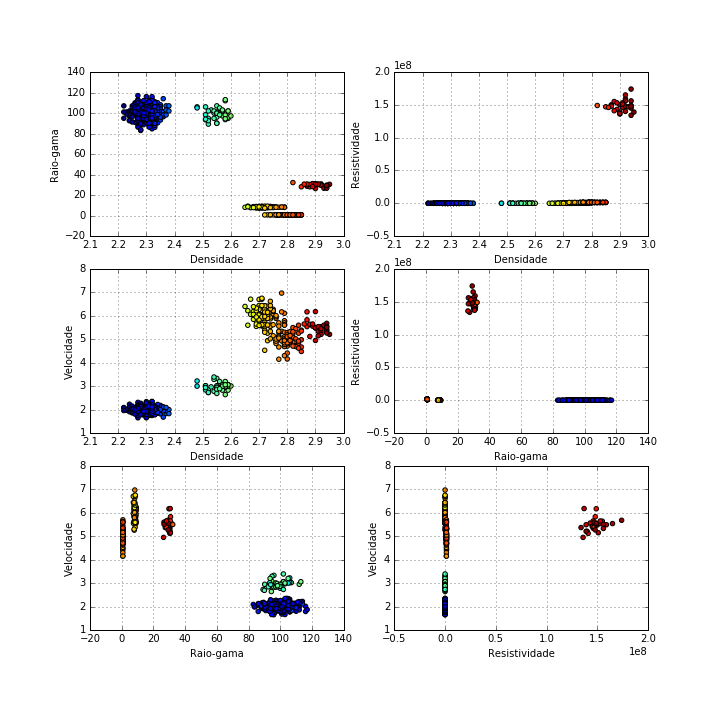
\includegraphics[scale=0.5]{Imagens/cluterpocoC2.png}
	}
	\caption{Agrupamento de dados do poço C2.}
	\label{clusterC2}
\end{figure} 

Na mesma forma, o agrupamento das classes de rochas é mais evidente, no gráfico de raio-gama por densidade, que evidencia os $5$ litotipos distintamente. E, da mesma maneira, o gráfico de velocidade por densidade.

\section{Treinamento}

A etapa de treinamento consiste em um ajuste de pesos dos neurônios da rede. Nesta fase, é identificado o neurônio que tem os valores dos pesos mais parecidos com os parâmetros de entrada da rede.  

\begin{figure}[H]
\centering
\subfigure[ref1][Iteração 1]{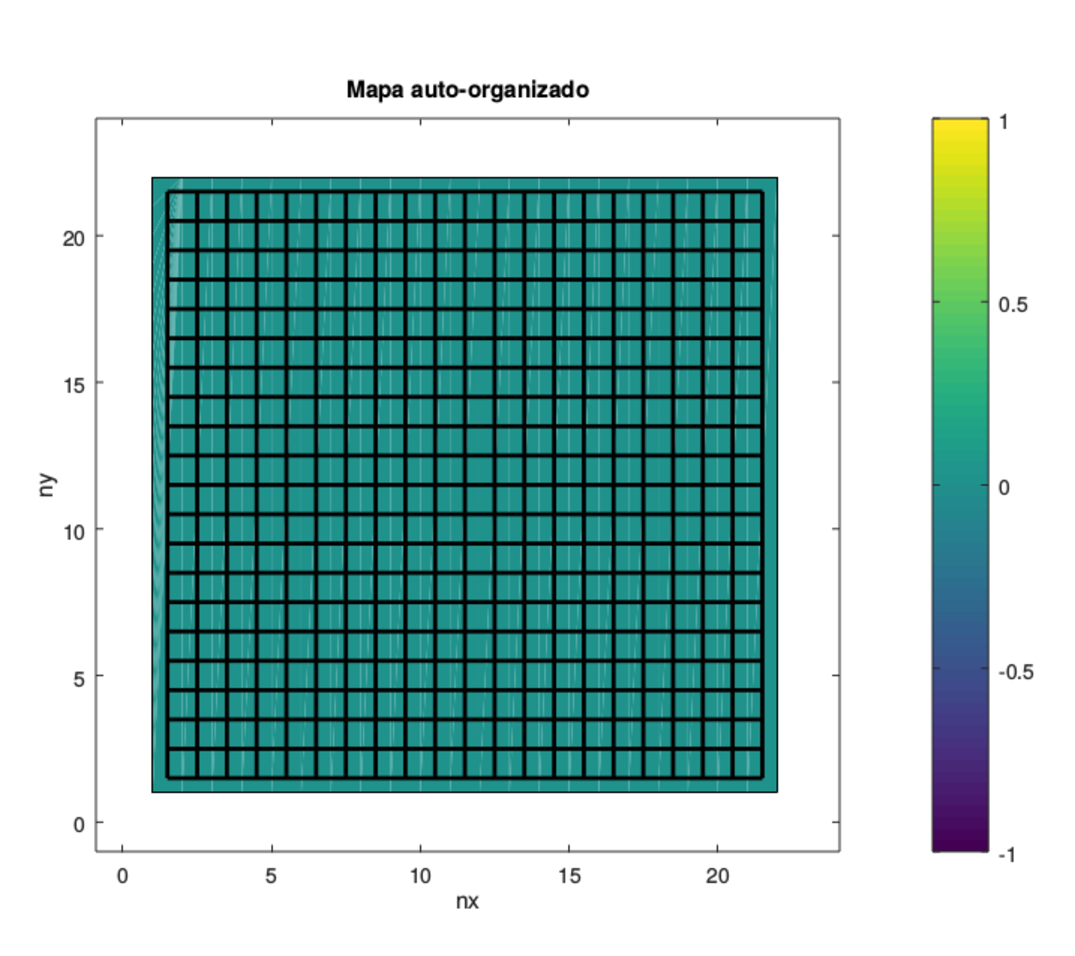
\includegraphics[width=7.0cm]{Imagens/SOM1_2d.pdf}}
\qquad
\subfigure[ref2][Iteração 5]{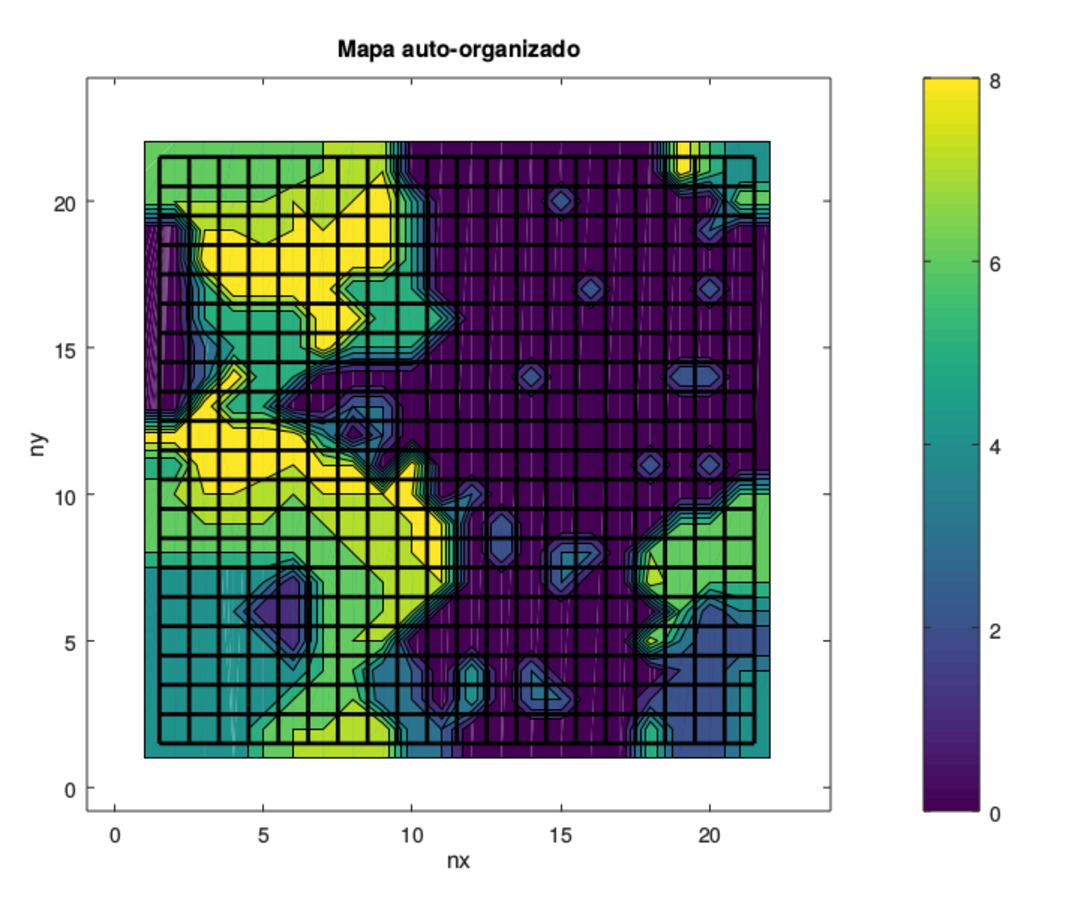
\includegraphics[width=7.0cm]{Imagens/SOM5_2d.pdf}}
\qquad
\subfigure[ref3][Iteração 100]{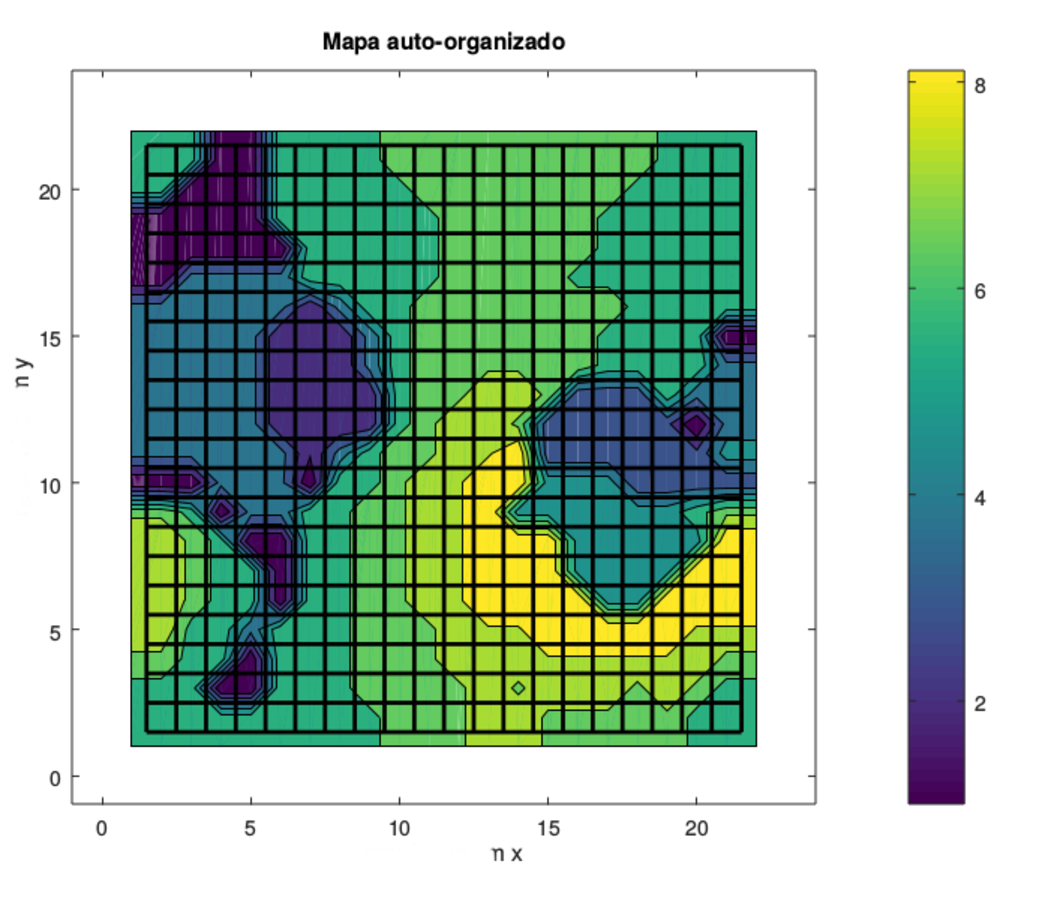
\includegraphics[width=7.0cm]{Imagens/SOM100_2d.pdf}}
\qquad
\subfigure[ref4][Iteração 1000]{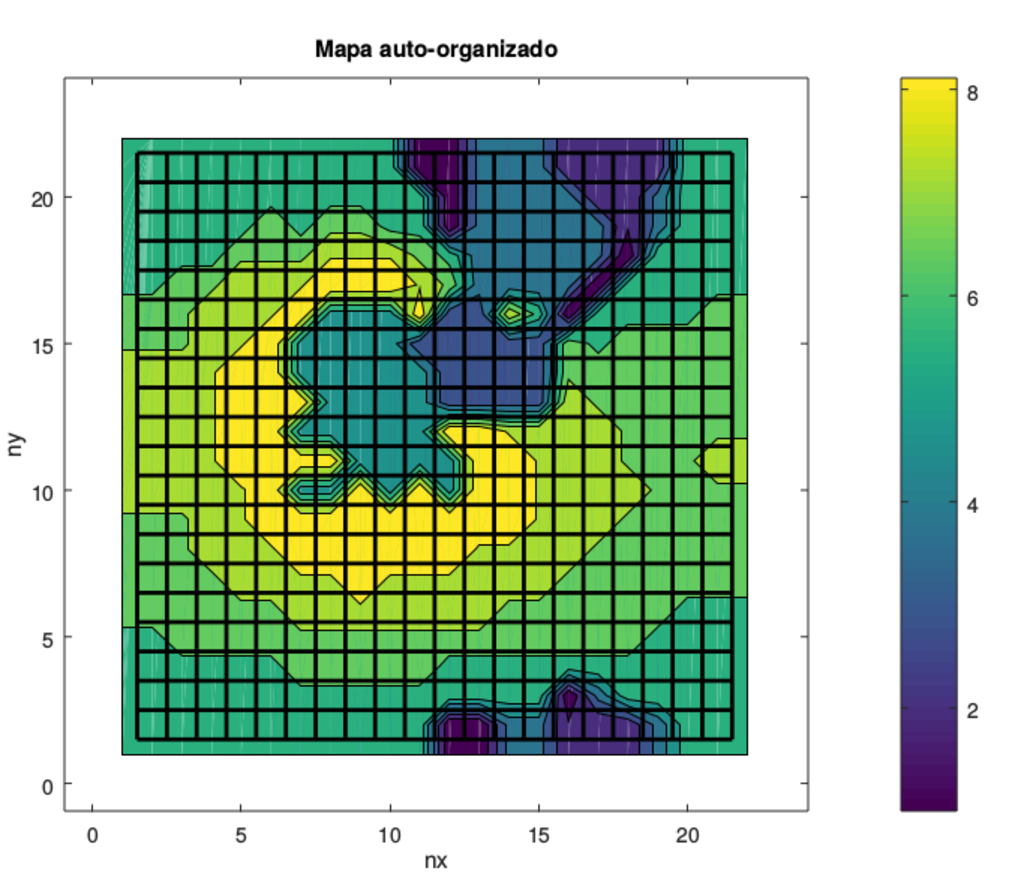
\includegraphics[width=7.0cm]{Imagens/SOM1000_2d.pdf}}
\qquad
\caption{Mapas auto-organizáveis e sua evolução temporal.}
\label{SOM}
\end{figure}

Os mapas da Fig. \ref{SOM} apresentam as zonas do hiperplano especializadas em identificar as classes de rochas. O código numérico $1$ representa folhelho, $2$ dolomita, $3$ diabásio, $4$ conglomerado, $5$ embasamento, $6$ mistura conglomerado/embasamento $75\%$, $7$ mistura conglomerado/embasamento $50\%$, $8$ mistura conglomerado/embasamento $25\%$.

A Fig. \ref{convergencia} apresenta o teste de convergência da rede neuronal.

\begin{figure}[H]
	\centering
	\setlength{\fboxsep}{8pt}
	\setlength{\fboxrule}{0.1pt}
	\fbox{
		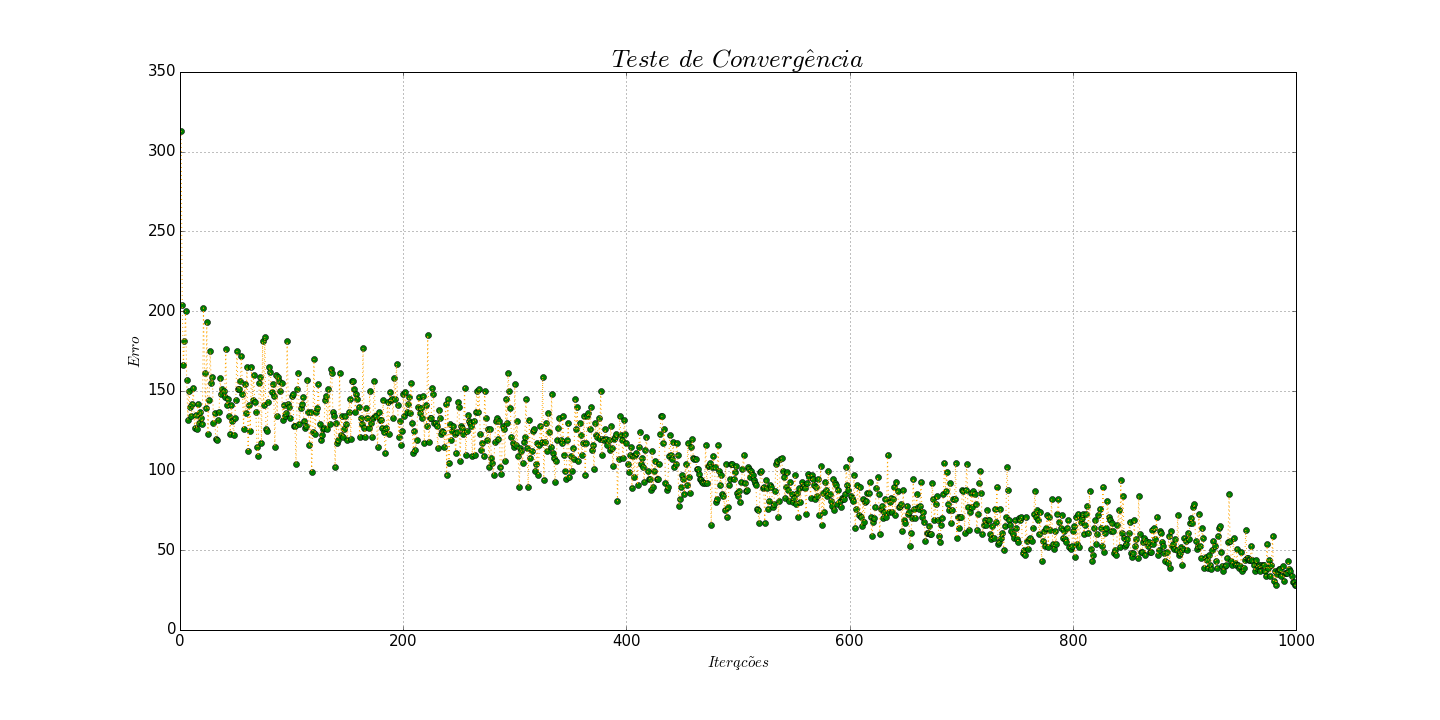
\includegraphics[scale=0.3]{Imagens/conv030917.png}
	}
	\caption{Teste de convergência da rede.}
	\label{convergencia}
\end{figure} 

O teste de convergência mostra que a rede se encontra estabilizada em  $1000$ iterações. Isto significa ser inócuo aumentar a iteração afim de diminuir o erro. 



\section{Identificação}



O QUE COLOCAR AQUI???







